\documentclass{article}

\usepackage{fullpage}
\usepackage{amsmath} 
\usepackage{xcolor}
\usepackage{xcolor} 
\newcommand{\lucas}[1]{\textbf{\textcolor{blue}{Lucas: #1}}}

\begin{document} 

\textbf{Principle statement} One sentence that succinctly explains the advance contained in this paper.


\begin{figure}
    %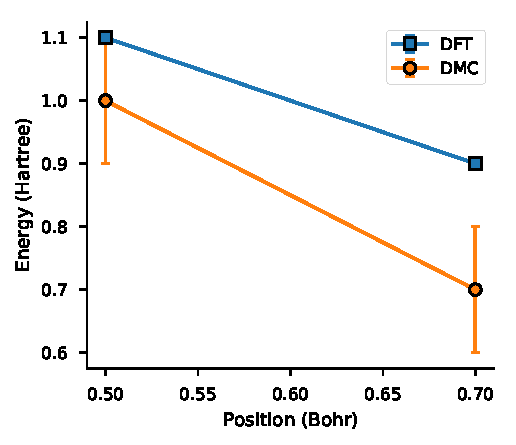
\includegraphics{../2_plots/fig_usefulname.pdf}
    \caption{4-5 figures. Each figure caption should give a short true statement that is shown by the figure. It's ok to start with hand-drawn figures.}
\end{figure}

\end{document} 